% ===================================================================
%  Week 9 — Session 2: Shape Descriptors, Invariance & Hierarchy
% ===================================================================
\documentclass[10pt,aspectratio=169]{beamer}
% ===================================================================
%  Shared Beamer preamble for "Practical Image Processing"
%  English slides. Compile with pdfLaTeX.
% ===================================================================

\usetheme{metropolis}
\usepackage[T1]{fontenc}
\usepackage[utf8]{inputenc}
\usepackage{lmodern}
\usepackage{listings}
\usepackage{tcolorbox}
\usepackage{fontawesome5}
\usepackage{booktabs}
\usepackage{amsmath,amssymb}
\usepackage{tikz}
\usepackage{pgfplots}
\pgfplotsset{compat=1.17}
\usetikzlibrary{arrows.meta,positioning,shapes.geometric,fit,backgrounds,matrix}
\tcbuselibrary{skins,breakable}

% ---- Palette --------------------------------------------------------
\definecolor{coursePrimary}{HTML}{1B4965}   % deep blue
\definecolor{courseAccent}{HTML}{E76F51}    % coral
\definecolor{courseGood}{HTML}{2A9D8F}      % teal
\definecolor{courseBad}{HTML}{C0392B}       % red
\definecolor{courseInfo}{HTML}{2980B9}      % blue
\definecolor{codeBg}{HTML}{F5F6FA}
\definecolor{codeKw}{HTML}{8E44AD}
\definecolor{codeStr}{HTML}{2A9D8F}
\definecolor{codeCom}{HTML}{7F8C8D}

\setbeamercolor{frametitle}{bg=coursePrimary}
\setbeamercolor{progress bar}{fg=courseAccent}
\setbeamercolor{alerted text}{fg=courseAccent}
\metroset{block=fill,sectionpage=progressbar,numbering=fraction}

% ---- Code listings (Python is built into listings) -----------------
\lstdefinestyle{course}{
  backgroundcolor=\color{codeBg},
  basicstyle=\ttfamily\scriptsize,
  keywordstyle=\color{codeKw}\bfseries,
  stringstyle=\color{codeStr},
  commentstyle=\color{codeCom}\itshape,
  numberstyle=\tiny\color{codeCom},
  numbers=left, numbersep=6pt,
  showstringspaces=false, breaklines=true, breakatwhitespace=true,
  tabsize=4, columns=fullflexible,
  frame=single, framesep=4pt, rulecolor=\color{gray!30},
  keepspaces=true, upquote=true, language=Python,
}
\lstset{style=course}
\lstdefinelanguage{bash}{
  keywords={cd,pip,python,venv,source,import}, sensitive=true,
  morecomment=[l]{\#}, morestring=[b]', morestring=[b]",
}

% ---- Reusable callout boxes ----------------------------------------
\newtcolorbox{goodbox}[1][Good practice]{colback=courseGood!8,colframe=courseGood,
  fonttitle=\bfseries,title={\faCheck~#1},boxrule=0.6pt,left=4pt,right=4pt,top=3pt,bottom=3pt}
\newtcolorbox{badbox}[1][Pitfall]{colback=courseBad!8,colframe=courseBad,
  fonttitle=\bfseries,title={\faTimes~#1},boxrule=0.6pt,left=4pt,right=4pt,top=3pt,bottom=3pt}
\newtcolorbox{infobox}[1][Note]{colback=courseInfo!8,colframe=courseInfo,
  fonttitle=\bfseries,title={\faInfoCircle~#1},boxrule=0.6pt,left=4pt,right=4pt,top=3pt,bottom=3pt}
\newtcolorbox{mathbox}[1][Math]{colback=coursePrimary!6,colframe=coursePrimary,
  fonttitle=\bfseries,title={\faCalculator~#1},boxrule=0.6pt,left=4pt,right=4pt,top=3pt,bottom=3pt}

\newcommand{\keyidea}[1]{\begin{alertblock}{Key idea}#1\end{alertblock}}
\newcommand{\term}[1]{\textbf{\color{coursePrimary}#1}}
\newcommand{\code}[1]{\lstinline[basicstyle=\ttfamily\small]|#1|}

% ---- A helper to draw a small pixel grid, cells shaded by value ----
% \pixelgrid{ {10,20,120,200,240}, {30,60,130,180,230}, ... }
\newcommand{\pixelgrid}[1]{%
  \begin{tikzpicture}[font=\scriptsize,scale=0.6]
    \foreach \row [count=\ry] in {#1} {
      \foreach \val [count=\cx] in \row {
        \draw[gray,fill=coursePrimary!8] (\cx,-\ry) rectangle ++(1,-1);
        \node at (\cx+0.5,-\ry-0.5) {\val};
      }
    }
  \end{tikzpicture}}


\title{Contours \& Shape Analysis}
\subtitle{Week 9 — Session 2: Descriptors, invariance \& hierarchy}
\author{Practical Image Processing}
\date{Lecture 9.2 \textbullet\ 60--70 min}

\begin{document}

\maketitle

\begin{frame}{Recap of Session 1}
  \begin{columns}[T]
    \begin{column}{0.58\textwidth}
      \begin{itemize}
        \item We traced \term{contours} from a binary mask and measured them: area (shoelace),
              perimeter, bounding box, rotated box, centroid.
        \item We filtered noise by \term{area} + \term{aspect ratio}, then cropped and ordered digits.
        \item \alert{Today:} numbers that \emph{describe} a shape and stay stable under rotation and
              scale — plus convex hulls, polygon approximation, and hierarchy (holes).
      \end{itemize}
    \end{column}
    \begin{column}{0.42\textwidth}
      \begin{alertblock}{DocScan milestone}
        Approximate a page's outline to \emph{4 corners} — the input to Week 11's perspective flatten.
      \end{alertblock}
    \end{column}
  \end{columns}
\end{frame}

\begin{frame}{Roadmap}\tableofcontents\end{frame}

% ==================================================================
\section{Convex hull \& convexity}
% ==================================================================

\begin{frame}{Convex hull \& convexity}
  \begin{columns}[T]
    \begin{column}{0.5\textwidth}\begin{center}
      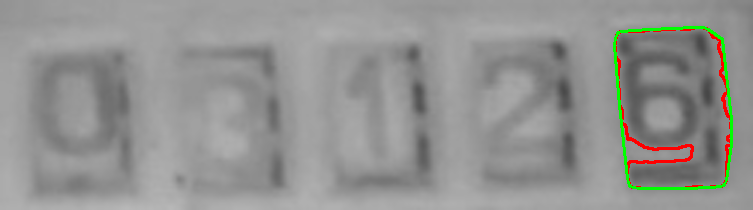
\includegraphics[width=0.95\linewidth]{../assets/hull.png}\\{\scriptsize contour (red) + convex hull (green)}
    \end{center}\end{column}
    \begin{column}{0.5\textwidth}
      \begin{itemize}
        \item \term{Convex hull}: the smallest convex shape enclosing the contour — a rubber band snapped around it.
        \item \code{hull = cv2.convexHull(c)} returns the hull points.
        \item \term{Convexity defects} (dents) reveal fingers, gaps, or the neck between touching objects.
        \item \term{Solidity} $=$ area $/$ hull area — how ``filled'' the shape is.
      \end{itemize}
    \end{column}
  \end{columns}
\end{frame}

\begin{frame}{Convexity defects}
  \begin{columns}[T]
    \begin{column}{0.45\textwidth}
    \begin{center}
    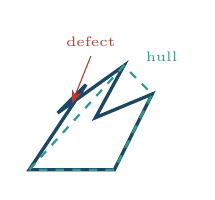
\begin{tikzpicture}[scale=0.6,font=\scriptsize]
      \draw[coursePrimary,very thick]
        (0,0)--(1.2,1.8)--(0.6,1.2)--(2,2.2)--(1.4,1.1)--(2.6,1.6)--(1.8,0)--cycle;
      \draw[courseGood,thick,dashed] (0,0)--(2,2.2)--(2.6,1.6)--(1.8,0)--cycle;
      \node[courseGood] at (2.8,2.4){\tiny hull};
      \draw[courseBad,-{Stealth[]}] (1.3,2.4) node[above]{\tiny defect} -- (0.9,1.4);
    \end{tikzpicture}
    \end{center}
    \end{column}
    \begin{column}{0.55\textwidth}
      \begin{itemize}\scriptsize
        \item A \term{defect} is a stretch where the contour dips away from its hull; its \emph{depth}
              measures how deep the dent is.
        \item \code{cv2.convexityDefects} returns start / end / farthest point / depth per dent.
        \item Classic use: count fingers on a hand, or detect where two coins touch (a deep neck).
      \end{itemize}
      \begin{infobox}[For DocScan]
        A clean page has \emph{few, shallow} defects — a strong ``this really is a rectangle'' cue.
      \end{infobox}
    \end{column}
  \end{columns}
\end{frame}

\begin{frame}{Worked example: solidity}
  \begin{columns}[T]
    \begin{column}{0.5\textwidth}
      \begin{mathbox}[Solidity]
        \[ \text{solidity}=\frac{\text{contour area}}{\text{hull area}} \]
        A solid convex blob $\rightarrow 1.0$; a dented / spiky shape $\rightarrow$ well below 1.
      \end{mathbox}
    \end{column}
    \begin{column}{0.5\textwidth}
      \begin{itemize}\scriptsize
        \item Star shape: area $=120$, hull area $=200 \Rightarrow$ solidity $=0.60$.
        \item Filled disc: area $\approx$ hull area $\Rightarrow$ solidity $\approx 0.98$.
        \item A digit ``8'' has a lowish solidity (two holes eat area); a filled ``1'' is high.
      \end{itemize}
      \begin{goodbox}
        Solidity is a cheap, scale-free feature — great for separating spiky junk from compact digits.
      \end{goodbox}
    \end{column}
  \end{columns}
\end{frame}

% ==================================================================
\section{Shape descriptors}
% ==================================================================

\begin{frame}{Descriptors: numbers that describe a shape}
  \begin{itemize}
    \item \term{Circularity} $= 4\pi\,\mathrm{area}/\mathrm{perimeter}^2$ (1 for a circle, lower for complex shapes).
    \item \term{Aspect ratio} $=w/h$, \term{extent} $=$ area$/$box area, \term{solidity} $=$ area$/$hull area.
    \item \term{Moments}: weighted sums that summarize a shape (centroid, orientation, spread).
  \end{itemize}
  \keyidea{A descriptor maps a whole shape to one small vector of numbers you can compare and threshold.}
\end{frame}

\begin{frame}{Circularity — derivation \& worked values}
  \begin{columns}[T]
    \begin{column}{0.52\textwidth}
      \begin{mathbox}[Why $4\pi A/P^2$?]
        A circle has $A=\pi r^2$, $P=2\pi r$, so
        \[ \frac{4\pi A}{P^2}=\frac{4\pi(\pi r^2)}{(2\pi r)^2}=\frac{4\pi^2 r^2}{4\pi^2 r^2}=1. \]
        Any other shape has more perimeter per unit area $\Rightarrow$ value $<1$.
      \end{mathbox}
    \end{column}
    \begin{column}{0.48\textwidth}
      \begin{itemize}\scriptsize
        \item Square: $A=s^2$, $P=4s\Rightarrow 4\pi s^2/16s^2=\pi/4\approx\mathbf{0.79}$.
        \item Equilateral triangle: $\approx\mathbf{0.60}$.
        \item Long thin scratch: $P$ huge, $A$ tiny $\Rightarrow \approx\mathbf{0.05}$.
      \end{itemize}
      \begin{infobox}[Also called]
        ``roundness'' or (its inverse) the \term{isoperimetric} ratio.
      \end{infobox}
    \end{column}
  \end{columns}
\end{frame}

\begin{frame}{Circularity separates shapes}
  \begin{center}
  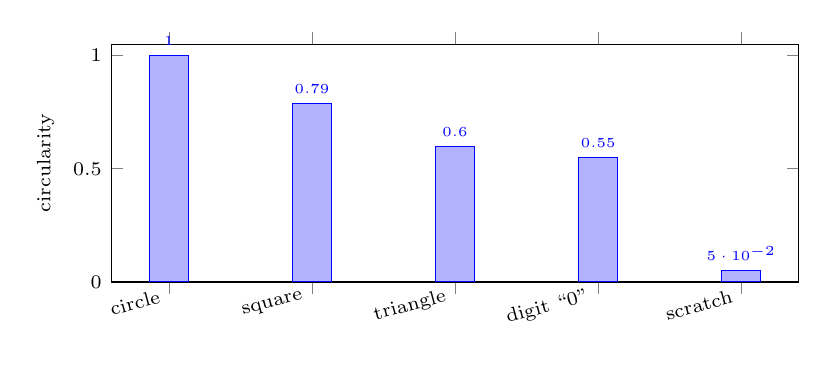
\begin{tikzpicture}
  \begin{axis}[
    ybar, width=0.85\textwidth, height=4.6cm,
    bar width=14pt, ymin=0, ymax=1.05,
    ylabel={circularity}, ylabel style={font=\scriptsize},
    symbolic x coords={circle,square,triangle,digit ``0'',scratch},
    xtick=data, xticklabel style={font=\scriptsize,rotate=15,anchor=east},
    ytick={0,0.5,1}, tick label style={font=\scriptsize},
    nodes near coords, nodes near coords style={font=\tiny},
    every axis plot/.append style={fill=coursePrimary!55,draw=coursePrimary}]
    \addplot coordinates {(circle,1.0) (square,0.79) (triangle,0.60) (digit ``0'',0.55) (scratch,0.05)};
  \end{axis}
  \end{tikzpicture}
  \end{center}
  \begin{itemize}\scriptsize
    \item One threshold ($\sim 0.2$) already rejects scratches; combine with area for robust filtering.
  \end{itemize}
\end{frame}

\begin{frame}{Extent, aspect ratio, solidity — side by side}
  \begin{center}\scriptsize
  \begin{tabular}{@{}lccl@{}}
    \toprule
    \textbf{Descriptor} & \textbf{Formula} & \textbf{Range} & \textbf{Reads as}\\
    \midrule
    Aspect ratio & $w/h$ & $0\!\to\!\infty$ & tall vs wide \\
    Extent & area $/(w\cdot h)$ & $0\!\to\!1$ & fills its box? \\
    Solidity & area $/$ hull area & $0\!\to\!1$ & dented / spiky? \\
    Circularity & $4\pi A/P^2$ & $0\!\to\!1$ & round vs jagged \\
    \bottomrule
  \end{tabular}
  \end{center}
  \begin{goodbox}
    All four are \emph{ratios} — unit-free and scale-free. A shape twice as big gives the same values.
  \end{goodbox}
\end{frame}

\begin{frame}{Moments: the raw material of descriptors}
  \begin{mathbox}[Image moments]
    \[ M_{pq}=\sum_{x}\sum_{y} x^{p}\,y^{q}\,I(x,y) \]
    $M_{00}$ = area/mass; $M_{10},M_{01}$ give the centroid $(\bar x,\bar y)=(M_{10}/M_{00},\,M_{01}/M_{00})$.
  \end{mathbox}
  \begin{itemize}
    \item \term{Central moments} $\mu_{pq}=\sum (x-\bar x)^p (y-\bar y)^q I$ subtract the centroid $\Rightarrow$ \term{translation-invariant}.
    \item \term{Normalized} central moments $\eta_{pq}=\mu_{pq}/\mu_{00}^{(1+(p+q)/2)}$ add \term{scale} invariance.
  \end{itemize}
\end{frame}

\begin{frame}{Orientation from second moments}
  \begin{columns}[T]
    \begin{column}{0.52\textwidth}
      \begin{mathbox}[Principal axis]
        \[ \theta=\tfrac12\arctan\!\Big(\frac{2\mu_{11}}{\mu_{20}-\mu_{02}}\Big) \]
        the angle of the shape's long axis — its ``tilt.''
      \end{mathbox}
    \end{column}
    \begin{column}{0.48\textwidth}
    \begin{center}
    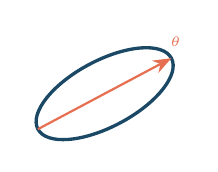
\begin{tikzpicture}[scale=0.6,font=\scriptsize]
      \draw[coursePrimary,very thick,rotate=28] (0,0) ellipse (1.6 and 0.7);
      \draw[courseAccent,thick,-{Stealth[]},rotate=28] (-1.6,0)--(1.6,0);
      \node[courseAccent] at (1.5,1.1){\tiny $\theta$};
    \end{tikzpicture}
    \end{center}
    \end{column}
  \end{columns}
  \begin{itemize}\scriptsize
    \item Second central moments $\mu_{20},\mu_{02},\mu_{11}$ describe how the mass \emph{spreads}.
    \item Orientation lets you de-rotate a tilted digit before recognition.
  \end{itemize}
\end{frame}

% ==================================================================
\section{Hu moments \& matching}
% ==================================================================

\begin{frame}{Hu moments: rotation/scale-invariant shape}
  \begin{itemize}
    \item \term{Hu moments}: 7 numbers built from normalized central moments, (nearly) invariant to
          \term{translation, rotation, and scale}.
    \item So the same shape gives the same descriptor regardless of where, how big, or how rotated it is.
    \item A classical alternative to a neural net for matching a shape to a template.
  \end{itemize}
  \begin{mathbox}[First Hu moment]
    \( h_1=\eta_{20}+\eta_{02} \) — spread about the centroid; the rest combine higher $\eta_{pq}$ to cancel rotation.
  \end{mathbox}
\end{frame}

\begin{frame}[fragile]{matchShapes: a shape similarity score}
\begin{lstlisting}[language=Python]
hu = cv2.HuMoments(cv2.moments(c)).flatten()   # 7-vector
# compare two contours directly:
score = cv2.matchShapes(c1, c2, cv2.CONTOURS_MATCH_I1, 0.0)
# score ~ 0  => very similar;  larger => more different
\end{lstlisting}
  \begin{itemize}
    \item Hu values span many orders of magnitude $\Rightarrow$ compare with a \term{log} transform (matchShapes does this internally).
    \item Match a query digit against templates ``0''--``9''; smallest score wins — a tiny, training-free classifier.
  \end{itemize}
\end{frame}

\begin{frame}{Worked example: same shape, moved \& rotated}
  \begin{columns}[T]
    \begin{column}{0.42\textwidth}
    \begin{center}
    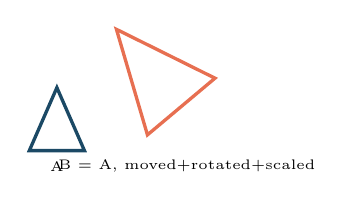
\begin{tikzpicture}[scale=0.5,font=\tiny]
      \draw[coursePrimary,very thick] (0,0)--(1.4,0)--(0.7,1.6)--cycle;
      \node at (0.7,-0.4){A};
      \begin{scope}[xshift=3cm,yshift=0.4cm,rotate=40,scale=1.6]
        \draw[courseAccent,very thick] (0,0)--(1.4,0)--(0.7,1.6)--cycle;
      \end{scope}
      \node at (4,-0.4){B = A, moved+rotated+scaled};
    \end{tikzpicture}
    \end{center}
    \end{column}
    \begin{column}{0.58\textwidth}
      \begin{itemize}\scriptsize
        \item Raw moments of A and B differ wildly (different position, size, angle).
        \item \term{Hu moments} of A and B are (almost) identical $\Rightarrow$ \code{matchShapes} score $\approx 0$.
        \item Small residual comes from rasterization, not from the transform.
      \end{itemize}
      \keyidea{Invariance means the descriptor answers ``what shape?'' not ``where / how big / which angle?''}
    \end{column}
  \end{columns}
\end{frame}

% ==================================================================
\section{Approximation \& hierarchy}
% ==================================================================

\begin{frame}{Contour approximation (polygon fitting)}
  \begin{columns}[T]
    \begin{column}{0.45\textwidth}
    \begin{center}
    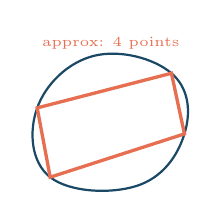
\begin{tikzpicture}[scale=0.55,font=\scriptsize]
      \draw[coursePrimary,thick] plot[smooth cycle,tension=0.7]
        coordinates{(0,0)(2,-0.2)(3.1,1)(2.8,2.4)(1,2.8)(-0.3,1.6)};
      \draw[courseAccent,very thick] (0,0)--(3.1,1)--(2.8,2.4)--(-0.3,1.6)--cycle;
      \node[courseAccent] at (1.4,3.1){\tiny approx: 4 points};
    \end{tikzpicture}
    \end{center}
    \end{column}
    \begin{column}{0.55\textwidth}
      \begin{itemize}\scriptsize
        \item \code{approxPolyDP(c, eps, True)} simplifies a contour to fewer points within a tolerance \code{eps}.
        \item Pick \code{eps} as a fraction of perimeter: \code{eps = 0.02*cv2.arcLength(c,True)}.
        \item A page/document boundary $\rightarrow$ approximates to \emph{4 points} $=$ the corners.
      \end{itemize}
      \keyidea{Approximating the page contour to a quadrilateral is how DocScan finds the page's corners.}
    \end{column}
  \end{columns}
\end{frame}

\begin{frame}{Douglas--Peucker: how the simplification works}
  \begin{center}
  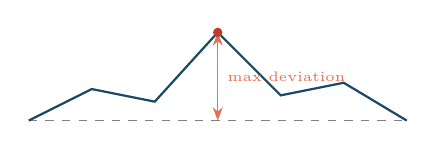
\begin{tikzpicture}[scale=0.8,font=\scriptsize]
    \draw[gray,dashed] (0,0)--(6,0);
    \draw[coursePrimary,thick] (0,0)--(1,0.5)--(2,0.3)--(3,1.4)--(4,0.4)--(5,0.6)--(6,0);
    \draw[courseAccent,{Stealth[]}-{Stealth[]}] (3,0) -- (3,1.4);
    \node[courseAccent,right] at (3,0.7){\tiny max deviation};
    \node[fill=courseBad,circle,inner sep=1.2pt] at (3,1.4){};
  \end{tikzpicture}
  \end{center}
  \begin{enumerate}
    \item Draw a line from the first to the last point; find the point farthest from it.
    \item If that distance $>$ \code{eps}, keep the point and recurse on the two halves.
    \item Otherwise discard all points between — a straight segment is enough.
  \end{enumerate}
  \begin{infobox}[Tuning]
    Bigger \code{eps} $\Rightarrow$ fewer points (coarser). Too big and a rectangle loses a corner.
  \end{infobox}
\end{frame}

\begin{frame}{DocScan: page $\rightarrow$ 4 corners}
  \begin{itemize}
    \item Take the \emph{largest} external contour (the page), approximate it, and \emph{require} 4 points.
    \item If the approximation gives 4 points $\rightarrow$ you have the page corners; order them TL, TR, BR, BL.
    \item Those 4 corners feed the perspective correction in Week 11 — the DocScan ``flatten'' step.
  \end{itemize}
  \begin{badbox}
    Shadows or a busy background can make the ``page'' contour non-quadrilateral. Guard: check area,
    convexity, and that exactly 4 points came back before trusting it.
  \end{badbox}
\end{frame}

\begin{frame}{Contour hierarchy (holes)}
  \begin{columns}[T]
    \begin{column}{0.42\textwidth}
    \begin{center}
    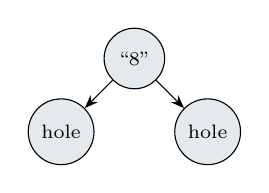
\begin{tikzpicture}[font=\scriptsize,node distance=5mm,
        n/.style={draw,circle,fill=coursePrimary!12,minimum size=6.5mm},
        a/.style={-{Stealth[]}}]
      \node[n](o){``8''};
      \node[n,below left=of o](h1){hole};
      \node[n,below right=of o](h2){hole};
      \draw[a](o)--(h1);\draw[a](o)--(h2);
    \end{tikzpicture}\\{\scriptsize outer contour + 2 inner (holes)}
    \end{center}
    \end{column}
    \begin{column}{0.58\textwidth}
      \begin{itemize}\scriptsize
        \item \term{RETR\_TREE} returns a \code{hierarchy} array: \code{[next, prev, first\_child, parent]} per contour.
        \item A ``0'' has one hole; ``8'' has two; ``1'' has none — a cheap, discriminative feature.
        \item For plain digit cropping, \term{RETR\_EXTERNAL} (outer only) is usually enough.
      \end{itemize}
    \end{column}
  \end{columns}
\end{frame}

\begin{frame}{Counting holes as a feature}
  \begin{center}\scriptsize
  \begin{tabular}{@{}cccccc@{}}
    \toprule
    Digit & 1 & 4 & 6 & 8 & 0 \\
    \midrule
    \# holes & 0 & 0/1 & 1 & 2 & 1 \\
    \bottomrule
  \end{tabular}
  \end{center}
  \begin{itemize}
    \item Count children of a contour in the hierarchy $\Rightarrow$ number of enclosed holes.
    \item Combined with solidity and aspect ratio, holes alone already split many digit classes.
    \item Font-dependent (a closed ``4'') — a hint, not a full classifier.
  \end{itemize}
\end{frame}

% ==================================================================
\section{Deep dive}
% ==================================================================

\begin{frame}{Counting \& measuring real objects}
  \begin{itemize}
    \item Count $=$ number of valid contours after filtering — cells, coins, parts, digits.
    \item Measure $=$ area / length / diameter per contour, converted to real units via a known scale.
    \item This is the backbone of industrial inspection and microscopy — pure classical vision.
  \end{itemize}
  \begin{goodbox}
    A calibrated pixel-to-mm ratio turns contour measurements into real-world dimensions.
  \end{goodbox}
\end{frame}

\begin{frame}{Worked example: pixel $\rightarrow$ millimetre}
  \begin{columns}[T]
    \begin{column}{0.55\textwidth}
      \begin{mathbox}[Calibration]
        A ruler's 10\,mm reads as 200\,px $\Rightarrow$ scale $s=\dfrac{10}{200}=0.05$ mm/px.
      \end{mathbox}
      \begin{itemize}\scriptsize
        \item A part's contour: width $=120$\,px $\Rightarrow 120\times0.05=\mathbf{6.0}$\,mm.
        \item Area scales by $s^2$: $4000$\,px$^2\times0.05^2=\mathbf{10}$\,mm$^2$.
      \end{itemize}
    \end{column}
    \begin{column}{0.45\textwidth}
      \begin{badbox}
        Area uses $s^2$, not $s$. Forgetting the square is the classic calibration bug.
      \end{badbox}
    \end{column}
  \end{columns}
\end{frame}

\begin{frame}{Robustness: the real-world contour mess}
  \begin{itemize}
    \item Contours are only as good as the binary mask — garbage in, garbage out.
    \item Broken digit $\rightarrow$ two contours; merged digits $\rightarrow$ one. Fix upstream (Weeks 7--8).
    \item Always filter by shape \emph{and} sanity-check the count on real data.
  \end{itemize}
  \begin{badbox}
    Don't trust the contour count blindly — a shadow or a smudge can add or merge objects.
  \end{badbox}
\end{frame}

\begin{frame}[fragile]{Contours in code — the full loop}
\begin{lstlisting}[language=Python]
cnts, _ = cv2.findContours(binary, cv2.RETR_EXTERNAL, cv2.CHAIN_APPROX_SIMPLE)
digits = []
for c in cnts:
    x, y, w, h = cv2.boundingRect(c)
    if cv2.contourArea(c) > 200 and 0.2 < w/h < 1.2:   # keep digit-like
        digits.append((x, gray[y:y+h, x:x+w]))
digits = [img for x, img in sorted(digits)]            # left-to-right
\end{lstlisting}
  Segment $\rightarrow$ contour $\rightarrow$ filter $\rightarrow$ crop $\rightarrow$ order. The DocScan hand-off, in seven lines.
\end{frame}

\begin{frame}{Fourier descriptors (brief)}
  \begin{itemize}
    \item Represent a contour as a complex signal $z_k=x_k+iy_k$ and take its Fourier transform (Week 6 again).
    \item Low-frequency coefficients $=$ overall shape; high $=$ fine boundary detail.
    \item Normalizing the coefficients gives \term{translation / rotation / scale} invariance, like Hu moments.
    \item Keeping a few coefficients gives a compact, robust descriptor for matching.
  \end{itemize}
\end{frame}

\begin{frame}{Shape analysis $\rightarrow$ recognition}
  \begin{itemize}
    \item Hu moments / Fourier descriptors can classify simple shapes with \emph{no} training.
    \item For digits, hand-crafted descriptors work but a CNN (Week 13) is more accurate.
    \item The pipeline is the same: segment $\rightarrow$ contour/crop $\rightarrow$ describe/classify.
  \end{itemize}
  \keyidea{Contours give clean, isolated objects; classical descriptors or a CNN then name them.}
\end{frame}

% ==================================================================
\section{In-class exercise}
% ==================================================================

\begin{frame}{\faPen~In-class exercise (12 min)}
  \begin{infobox}[Pick descriptors for a task]
    You must sort a tray of mixed hardware from one photo: round washers, hex nuts, and long screws.
  \end{infobox}
  \begin{enumerate}
    \item Which \emph{single} descriptor best separates washers from screws? Why?
    \item Which distinguishes a washer (has a hole) from a solid disc?
    \item Two nuts overlap and merge into one contour — which cue (defects? solidity?) flags it?
    \item Which of your chosen descriptors survive the camera zooming in $2\times$?
  \end{enumerate}
\end{frame}

\begin{frame}{\faPen~Debrief}
  \begin{itemize}
    \item Washer vs screw: \term{circularity} (or aspect ratio) — screws are long and thin, washers round.
    \item Washer vs disc: hole count from the \term{hierarchy}, or low \term{solidity} / extent.
    \item Merged nuts: a deep \term{convexity defect} at the neck; solidity drops below a single nut's.
    \item Zoom-safe: all \emph{ratio} descriptors (circularity, solidity, extent, Hu) are scale-free. \checkmark
  \end{itemize}
  \keyidea{Choose descriptors by the invariances the task needs — not by habit.}
\end{frame}

% ==================================================================
\section{Wrap-up \& deliverable}
% ==================================================================

\begin{frame}{What you should now be able to do}
  \begin{itemize}
    \item Compute convex hull, convexity defects, and solidity.
    \item Compute shape descriptors (circularity, extent, solidity, aspect ratio) and explain their invariances.
    \item Use moments for centroid \& orientation; use Hu moments / \code{matchShapes} for invariant matching.
    \item Approximate a page contour to 4 corners; read a contour hierarchy to count holes.
  \end{itemize}
\end{frame}

\begin{frame}{This week's deliverable}
  \begin{alertblock}{Due before Week 10 (see \code{project/})}
    \begin{enumerate}
      \item Find and draw contours on a cleaned meter binary; report each digit's area \& bounding box.
      \item Filter out noise contours with an area + aspect-ratio rule; verify the count.
      \item Crop each digit by its bounding box and output them ordered left-to-right.
      \item Compute one \term{invariant} descriptor per digit (circularity or a Hu moment) and tabulate it.
      \item Bonus: approximate a document's outer contour to its 4 corners.
    \end{enumerate}
  \end{alertblock}
\end{frame}

\begin{frame}[standout]
  From outlines to identities.\\[4pt]
  \normalsize Describe, make invariant, approximate, and match — the classical road to reading a shape.
\end{frame}

\end{document}
